\documentclass[twoside]{book}

% Packages required by doxygen
\usepackage{fixltx2e}
\usepackage{calc}
\usepackage{doxygen}
\usepackage[export]{adjustbox} % also loads graphicx
\usepackage{graphicx}
\usepackage[utf8]{inputenc}
\usepackage{makeidx}
\usepackage{multicol}
\usepackage{multirow}
\PassOptionsToPackage{warn}{textcomp}
\usepackage{textcomp}
\usepackage[nointegrals]{wasysym}
\usepackage[table]{xcolor}

% Font selection
\usepackage[T1]{fontenc}
\usepackage[scaled=.90]{helvet}
\usepackage{courier}
\usepackage{amssymb}
\usepackage{sectsty}
\renewcommand{\familydefault}{\sfdefault}
\allsectionsfont{%
  \fontseries{bc}\selectfont%
  \color{darkgray}%
}
\renewcommand{\DoxyLabelFont}{%
  \fontseries{bc}\selectfont%
  \color{darkgray}%
}
\newcommand{\+}{\discretionary{\mbox{\scriptsize$\hookleftarrow$}}{}{}}

% Page & text layout
\usepackage{geometry}
\geometry{%
  a4paper,%
  top=2.5cm,%
  bottom=2.5cm,%
  left=2.5cm,%
  right=2.5cm%
}
\tolerance=750
\hfuzz=15pt
\hbadness=750
\setlength{\emergencystretch}{15pt}
\setlength{\parindent}{0cm}
\setlength{\parskip}{3ex plus 2ex minus 2ex}
\makeatletter
\renewcommand{\paragraph}{%
  \@startsection{paragraph}{4}{0ex}{-1.0ex}{1.0ex}{%
    \normalfont\normalsize\bfseries\SS@parafont%
  }%
}
\renewcommand{\subparagraph}{%
  \@startsection{subparagraph}{5}{0ex}{-1.0ex}{1.0ex}{%
    \normalfont\normalsize\bfseries\SS@subparafont%
  }%
}
\makeatother

% Headers & footers
\usepackage{fancyhdr}
\pagestyle{fancyplain}
\fancyhead[LE]{\fancyplain{}{\bfseries\thepage}}
\fancyhead[CE]{\fancyplain{}{}}
\fancyhead[RE]{\fancyplain{}{\bfseries\leftmark}}
\fancyhead[LO]{\fancyplain{}{\bfseries\rightmark}}
\fancyhead[CO]{\fancyplain{}{}}
\fancyhead[RO]{\fancyplain{}{\bfseries\thepage}}
\fancyfoot[LE]{\fancyplain{}{}}
\fancyfoot[CE]{\fancyplain{}{}}
\fancyfoot[RE]{\fancyplain{}{\bfseries\scriptsize Generated by Doxygen }}
\fancyfoot[LO]{\fancyplain{}{\bfseries\scriptsize Generated by Doxygen }}
\fancyfoot[CO]{\fancyplain{}{}}
\fancyfoot[RO]{\fancyplain{}{}}
\renewcommand{\footrulewidth}{0.4pt}
\renewcommand{\chaptermark}[1]{%
  \markboth{#1}{}%
}
\renewcommand{\sectionmark}[1]{%
  \markright{\thesection\ #1}%
}

% Indices & bibliography
\usepackage{natbib}
\usepackage[titles]{tocloft}
\setcounter{tocdepth}{3}
\setcounter{secnumdepth}{5}
\makeindex

% Hyperlinks (required, but should be loaded last)
\usepackage{ifpdf}
\ifpdf
  \usepackage[pdftex,pagebackref=true]{hyperref}
\else
  \usepackage[ps2pdf,pagebackref=true]{hyperref}
\fi
\hypersetup{%
  colorlinks=true,%
  linkcolor=blue,%
  citecolor=blue,%
  unicode%
}

% Custom commands
\newcommand{\clearemptydoublepage}{%
  \newpage{\pagestyle{empty}\cleardoublepage}%
}

\usepackage{caption}
\captionsetup{labelsep=space,justification=centering,font={bf},singlelinecheck=off,skip=4pt,position=top}

%===== C O N T E N T S =====

\begin{document}

% Titlepage & ToC
\hypersetup{pageanchor=false,
             bookmarksnumbered=true,
             pdfencoding=unicode
            }
\pagenumbering{alph}
\begin{titlepage}
\vspace*{7cm}
\begin{center}%
{\Large TP A\+OD }\\
\vspace*{1cm}
{\large Generated by Doxygen 1.8.13}\\
\end{center}
\end{titlepage}
\clearemptydoublepage
\pagenumbering{roman}
\tableofcontents
\clearemptydoublepage
\pagenumbering{arabic}
\hypersetup{pageanchor=true}

%--- Begin generated contents ---
\chapter{Class Index}
\section{Class List}
Here are the classes, structs, unions and interfaces with brief descriptions\+:\begin{DoxyCompactList}
\item\contentsline{section}{\hyperlink{structfichier}{fichier} }{\pageref{structfichier}}{}
\end{DoxyCompactList}

\chapter{File Index}
\section{File List}
Here is a list of all documented files with brief descriptions\+:\begin{DoxyCompactList}
\item\contentsline{section}{src/\hyperlink{algo__1_8c}{algo\+\_\+1.\+c} }{\pageref{algo__1_8c}}{}
\item\contentsline{section}{src/{\bfseries algo\+\_\+1.\+h} }{\pageref{algo__1_8h}}{}
\item\contentsline{section}{src/\hyperlink{computePatchOpt_8c}{compute\+Patch\+Opt.\+c} }{\pageref{computePatchOpt_8c}}{}
\item\contentsline{section}{src/\hyperlink{outils_8c}{outils.\+c} }{\pageref{outils_8c}}{}
\item\contentsline{section}{src/{\bfseries outils.\+h} }{\pageref{outils_8h}}{}
\end{DoxyCompactList}

\chapter{Class Documentation}
\hypertarget{structfichier}{}\section{fichier Struct Reference}
\label{structfichier}\index{fichier@{fichier}}
\subsection*{Public Attributes}
\begin{DoxyCompactItemize}
\item 
\mbox{\Hypertarget{structfichier_a569e06bfd23afa16c1af5374a1f7d4cf}\label{structfichier_a569e06bfd23afa16c1af5374a1f7d4cf}} 
char $\ast$ {\bfseries ptr}
\item 
\mbox{\Hypertarget{structfichier_afa26ad05fd496adfb5c7094cfd70e44d}\label{structfichier_afa26ad05fd496adfb5c7094cfd70e44d}} 
int {\bfseries nbr\+\_\+lines}
\item 
\mbox{\Hypertarget{structfichier_a3a07f98abefca3b78b4747c12d14eb80}\label{structfichier_a3a07f98abefca3b78b4747c12d14eb80}} 
int $\ast$ {\bfseries tab\+\_\+size\+\_\+line}
\item 
\mbox{\Hypertarget{structfichier_a3df4c0289a8cb15d7945c8d15d2bb279}\label{structfichier_a3df4c0289a8cb15d7945c8d15d2bb279}} 
char $\ast$$\ast$ {\bfseries tab\+\_\+ligne}
\end{DoxyCompactItemize}


The documentation for this struct was generated from the following file\+:\begin{DoxyCompactItemize}
\item 
src/outils.\+h\end{DoxyCompactItemize}

\chapter{File Documentation}
\hypertarget{algo__1_8c}{}\section{src/algo\+\_\+1.c File Reference}
\label{algo__1_8c}\index{src/algo\+\_\+1.\+c@{src/algo\+\_\+1.\+c}}
{\ttfamily \#include \char`\"{}algo\+\_\+1.\+h\char`\"{}}\newline
{\ttfamily \#include $<$time.\+h$>$}\newline
Include dependency graph for algo\+\_\+1.\+c\+:
\nopagebreak
\begin{figure}[H]
\begin{center}
\leavevmode
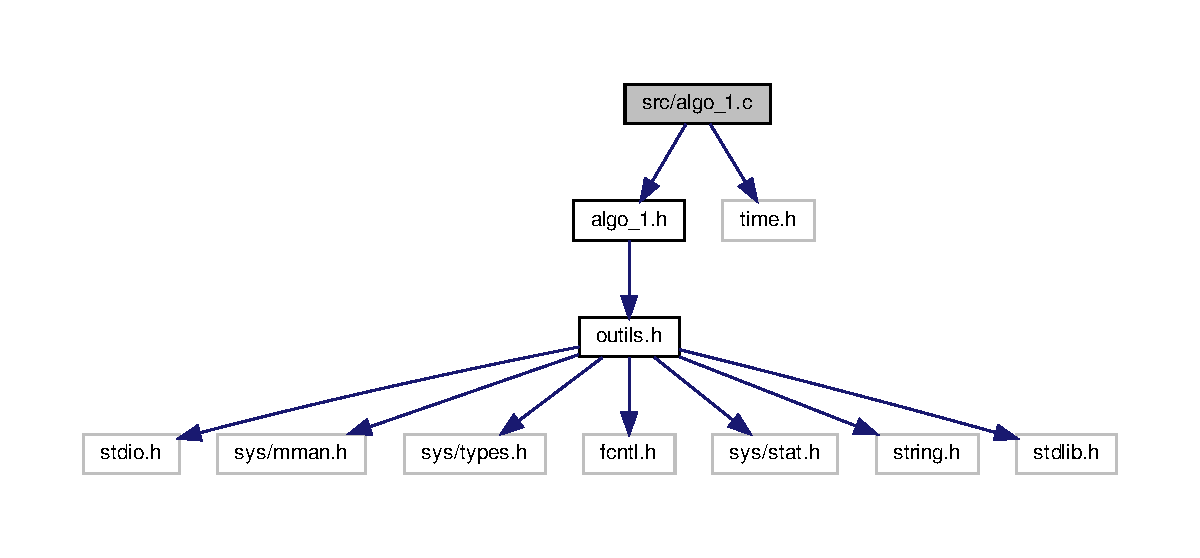
\includegraphics[width=350pt]{algo__1_8c__incl}
\end{center}
\end{figure}
\subsection*{Functions}
\begin{DoxyCompactItemize}
\item 
void \hyperlink{algo__1_8c_ab2f366ea409e581dad1e4ad8fb7efc4e}{write\+\_\+patch\+\_\+recur} (int $\ast$$\ast$mat, int i, int j, F\+I\+LE $\ast$patch, \hyperlink{structfichier}{fichier} src, \hyperlink{structfichier}{fichier} dst)
\item 
void \hyperlink{algo__1_8c_adb65578042b03445ffc67aa58088a9d5}{algo\+\_\+iter} (const char $\ast$F1, const char $\ast$F2, const char $\ast$P)
\begin{DoxyCompactList}\small\item\em Cette fonction récupère les fichiers, les traite selon des fonctions dans \hyperlink{outils_8c}{outils.\+c} et remplit le patch. \end{DoxyCompactList}\end{DoxyCompactItemize}
\subsection*{Variables}
\begin{DoxyCompactItemize}
\item 
\mbox{\Hypertarget{algo__1_8c_abb9aa376b5a18fad77633f41cef5e31e}\label{algo__1_8c_abb9aa376b5a18fad77633f41cef5e31e}} 
void $\ast$ {\bfseries ptr\+\_\+begin\+\_\+file}
\end{DoxyCompactItemize}


\subsection{Detailed Description}
\begin{DoxyAuthor}{Author}
Benjelloun hamza, Ait lahmouch Nadir 
\end{DoxyAuthor}


\subsection{Function Documentation}
\mbox{\Hypertarget{algo__1_8c_adb65578042b03445ffc67aa58088a9d5}\label{algo__1_8c_adb65578042b03445ffc67aa58088a9d5}} 
\index{algo\+\_\+1.\+c@{algo\+\_\+1.\+c}!algo\+\_\+iter@{algo\+\_\+iter}}
\index{algo\+\_\+iter@{algo\+\_\+iter}!algo\+\_\+1.\+c@{algo\+\_\+1.\+c}}
\subsubsection{\texorpdfstring{algo\+\_\+iter()}{algo\_iter()}}
{\footnotesize\ttfamily void algo\+\_\+iter (\begin{DoxyParamCaption}\item[{const char $\ast$}]{F1,  }\item[{const char $\ast$}]{F2,  }\item[{const char $\ast$}]{P }\end{DoxyParamCaption})}



Cette fonction récupère les fichiers, les traite selon des fonctions dans \hyperlink{outils_8c}{outils.\+c} et remplit le patch. 


\begin{DoxyParams}{Parameters}
{\em F1} & Notre fichier source qu\textquotesingle{}on va passer en paramètre \\
\hline
{\em F2} & Notre fichier Target qu\textquotesingle{}on va passer en paramètre \\
\hline
{\em P} & Notre fichier Patch qu\textquotesingle{}on va passer en paramètre \\
\hline
\end{DoxyParams}
\begin{DoxyReturn}{Returns}
Ne retourne rien, mais écrit dans le patch écrit en paramètre 
\end{DoxyReturn}
\mbox{\Hypertarget{algo__1_8c_ab2f366ea409e581dad1e4ad8fb7efc4e}\label{algo__1_8c_ab2f366ea409e581dad1e4ad8fb7efc4e}} 
\index{algo\+\_\+1.\+c@{algo\+\_\+1.\+c}!write\+\_\+patch\+\_\+recur@{write\+\_\+patch\+\_\+recur}}
\index{write\+\_\+patch\+\_\+recur@{write\+\_\+patch\+\_\+recur}!algo\+\_\+1.\+c@{algo\+\_\+1.\+c}}
\subsubsection{\texorpdfstring{write\+\_\+patch\+\_\+recur()}{write\_patch\_recur()}}
{\footnotesize\ttfamily void write\+\_\+patch\+\_\+recur (\begin{DoxyParamCaption}\item[{int $\ast$$\ast$}]{mat,  }\item[{int}]{i,  }\item[{int}]{j,  }\item[{F\+I\+LE $\ast$}]{patch,  }\item[{\hyperlink{structfichier}{fichier}}]{src,  }\item[{\hyperlink{structfichier}{fichier}}]{dst }\end{DoxyParamCaption})}


\begin{DoxyParams}{Parameters}
{\em mat} & La matrice qui mémorise les valeurs de tous les noeuds de notre graphe d\textquotesingle{}appel. \\
\hline
{\em i} & indexe qui renvoie aux lignes du fichier source \\
\hline
{\em j} & indexe qui renvoie aux lignes du fichier target \\
\hline
{\em patch} & Notre fichier patch qu\textquotesingle{}on remplit \\
\hline
{\em src} & Le fichier source \\
\hline
{\em dst} & Le fichier Destination \\
\hline
\end{DoxyParams}
\begin{DoxyReturn}{Returns}
Ne retourne rien, mais écrit dans le patch écrit en paramètre 
\end{DoxyReturn}

\hypertarget{computePatchOpt_8c}{}\section{src/compute\+Patch\+Opt.c File Reference}
\label{computePatchOpt_8c}\index{src/compute\+Patch\+Opt.\+c@{src/compute\+Patch\+Opt.\+c}}
{\ttfamily \#include \char`\"{}algo\+\_\+1.\+h\char`\"{}}\newline
{\ttfamily \#include $<$stdlib.\+h$>$}\newline
{\ttfamily \#include $<$assert.\+h$>$}\newline
{\ttfamily \#include $<$time.\+h$>$}\newline
Include dependency graph for compute\+Patch\+Opt.\+c\+:
\nopagebreak
\begin{figure}[H]
\begin{center}
\leavevmode
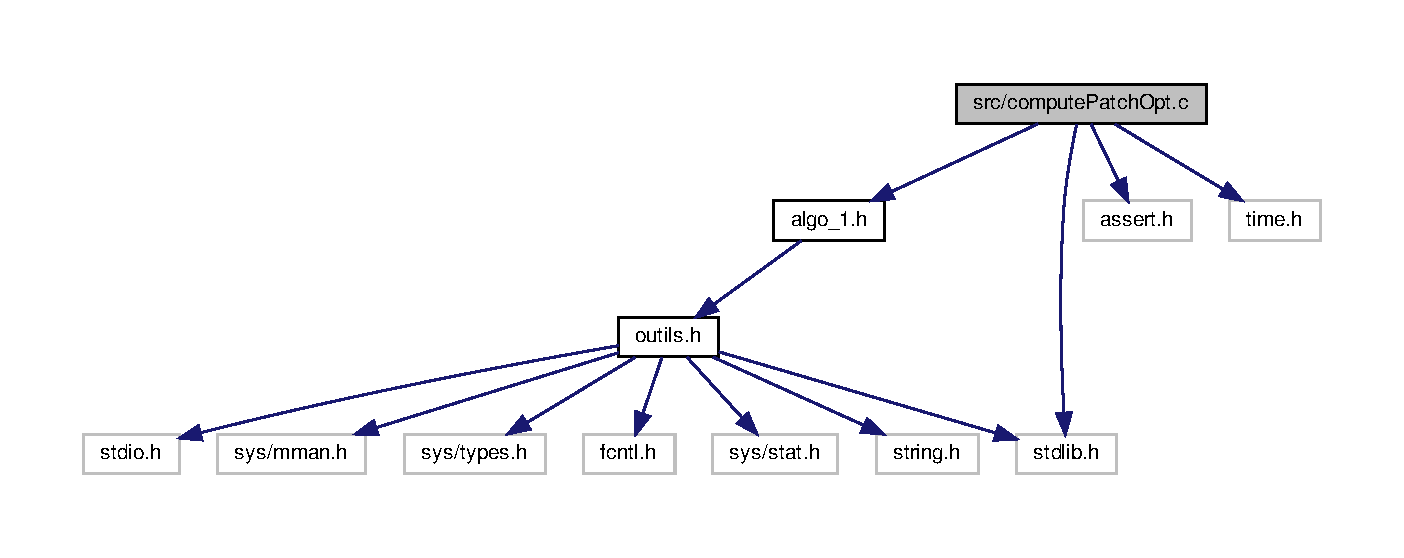
\includegraphics[width=350pt]{computePatchOpt_8c__incl}
\end{center}
\end{figure}
\subsection*{Functions}
\begin{DoxyCompactItemize}
\item 
int \hyperlink{computePatchOpt_8c_a91a3bbcc7eb26e8695255b2795d6e46f}{main} (int argc, char $\ast$argv\mbox{[}$\,$\mbox{]})
\end{DoxyCompactItemize}
\subsection*{Variables}
\begin{DoxyCompactItemize}
\item 
\mbox{\Hypertarget{computePatchOpt_8c_abb9aa376b5a18fad77633f41cef5e31e}\label{computePatchOpt_8c_abb9aa376b5a18fad77633f41cef5e31e}} 
void $\ast$ {\bfseries ptr\+\_\+begin\+\_\+file} = 0
\end{DoxyCompactItemize}


\subsection{Detailed Description}
\begin{DoxyAuthor}{Author}
Dorothée 
\end{DoxyAuthor}


\subsection{Function Documentation}
\mbox{\Hypertarget{computePatchOpt_8c_a91a3bbcc7eb26e8695255b2795d6e46f}\label{computePatchOpt_8c_a91a3bbcc7eb26e8695255b2795d6e46f}} 
\index{compute\+Patch\+Opt.\+c@{compute\+Patch\+Opt.\+c}!main@{main}}
\index{main@{main}!compute\+Patch\+Opt.\+c@{compute\+Patch\+Opt.\+c}}
\subsubsection{\texorpdfstring{main()}{main()}}
{\footnotesize\ttfamily void main (\begin{DoxyParamCaption}\item[{int}]{argc,  }\item[{char $\ast$}]{argv\mbox{[}$\,$\mbox{]} }\end{DoxyParamCaption})}


\begin{DoxyParams}{Parameters}
{\em argc} & Le fichier source \\
\hline
{\em argc} & Le fichier Destination \\
\hline
\end{DoxyParams}

\hypertarget{outils_8c}{}\section{src/outils.c File Reference}
\label{outils_8c}\index{src/outils.\+c@{src/outils.\+c}}
{\ttfamily \#include \char`\"{}outils.\+h\char`\"{}}\newline
Include dependency graph for outils.\+c\+:
\nopagebreak
\begin{figure}[H]
\begin{center}
\leavevmode
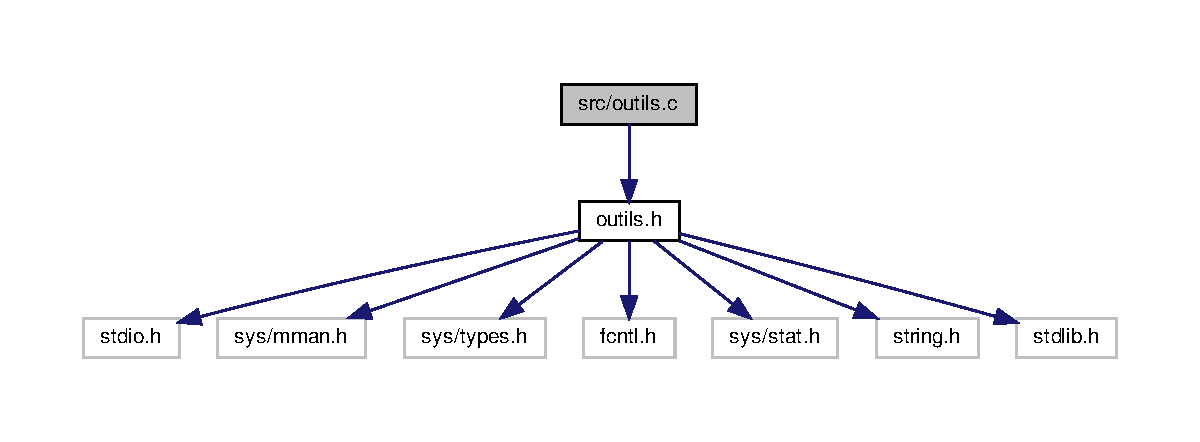
\includegraphics[width=350pt]{outils_8c__incl}
\end{center}
\end{figure}
\subsection*{Functions}
\begin{DoxyCompactItemize}
\item 
size\+\_\+t \hyperlink{outils_8c_a725c5803bf7a75d4d7986a6eb0707fc6}{get\+Filesize} (const char $\ast$filename)
\begin{DoxyCompactList}\small\item\em Retourne la taille du fichier qu\textquotesingle{}on passe en paramètre. \end{DoxyCompactList}\item 
void $\ast$ \hyperlink{outils_8c_a0adb6932c68f4e692a6250605c30d81f}{convert\+\_\+file\+\_\+to\+\_\+table} (const char $\ast$filename)
\begin{DoxyCompactList}\small\item\em Convertit un fichier en une table en utilisant mmap. \end{DoxyCompactList}\item 
int \hyperlink{outils_8c_a3d6a3d7631a318378e5be8194076e340}{get\+\_\+nbr\+\_\+lines} (char $\ast$ptr\+\_\+file)
\begin{DoxyCompactList}\small\item\em Calcule et donne le nombre de ligne dans un fichier. \end{DoxyCompactList}\item 
\hyperlink{structfichier}{fichier} \hyperlink{outils_8c_a07333c321cce76c9744973c4b667dbbd}{lines} (char $\ast$ptr\+\_\+file)
\begin{DoxyCompactList}\small\item\em Remplit les champs de la struture fichier qu\textquotesingle{}on a implémenté (voir \hyperlink{outils_8h_source}{outils.\+h}) \end{DoxyCompactList}\item 
int \hyperlink{outils_8c_af4d25f3f1939424ad4be8e5e45c63d06}{min\+\_\+2} (int a, int b)
\begin{DoxyCompactList}\small\item\em Calcule le min de deux nombres. \end{DoxyCompactList}\item 
int \hyperlink{outils_8c_a81e308f0a31421e49d46cc1772eb0a1f}{min\+\_\+3} (int a, int b, int c)
\begin{DoxyCompactList}\small\item\em Calcule le min de trois nombres. \end{DoxyCompactList}\item 
\mbox{\Hypertarget{outils_8c_adcaa349924a3d0300b9f8c331023d9ac}\label{outils_8c_adcaa349924a3d0300b9f8c331023d9ac}} 
int {\bfseries sum} (int $\ast$T, int size)
\item 
int \hyperlink{outils_8c_acff80b575580eb0622fdac28dad29805}{C} (int n, int m, \hyperlink{structfichier}{fichier} f1, \hyperlink{structfichier}{fichier} f2)
\begin{DoxyCompactList}\small\item\em Cette fonction calcule le coût pour transformer une lign A\+\_\+i en la ligne B\+\_\+j. \end{DoxyCompactList}\end{DoxyCompactItemize}
\subsection*{Variables}
\begin{DoxyCompactItemize}
\item 
\mbox{\Hypertarget{outils_8c_abb9aa376b5a18fad77633f41cef5e31e}\label{outils_8c_abb9aa376b5a18fad77633f41cef5e31e}} 
void $\ast$ {\bfseries ptr\+\_\+begin\+\_\+file}
\end{DoxyCompactItemize}


\subsection{Detailed Description}
\begin{DoxyAuthor}{Author}
Benjelloun hamza, Ait lahmouch Nadir 
\end{DoxyAuthor}


\subsection{Function Documentation}
\mbox{\Hypertarget{outils_8c_acff80b575580eb0622fdac28dad29805}\label{outils_8c_acff80b575580eb0622fdac28dad29805}} 
\index{outils.\+c@{outils.\+c}!C@{C}}
\index{C@{C}!outils.\+c@{outils.\+c}}
\subsubsection{\texorpdfstring{C()}{C()}}
{\footnotesize\ttfamily int C (\begin{DoxyParamCaption}\item[{int}]{n,  }\item[{int}]{m,  }\item[{\hyperlink{structfichier}{fichier}}]{f1,  }\item[{\hyperlink{structfichier}{fichier}}]{f2 }\end{DoxyParamCaption})}



Cette fonction calcule le coût pour transformer une lign A\+\_\+i en la ligne B\+\_\+j. 


\begin{DoxyParams}{Parameters}
{\em n} & indice de la ligne du fichier source qu\textquotesingle{}on veut transformer \\
\hline
{\em m} & indice de la ligne du fichier target \\
\hline
{\em f1} & Fichier Source \\
\hline
{\em f2} & Fichier Target \\
\hline
\end{DoxyParams}
\begin{DoxyReturn}{Returns}
Un int qui est le coût pour transformer une lign A\+\_\+i en la ligne B\+\_\+j 
\end{DoxyReturn}
\mbox{\Hypertarget{outils_8c_a0adb6932c68f4e692a6250605c30d81f}\label{outils_8c_a0adb6932c68f4e692a6250605c30d81f}} 
\index{outils.\+c@{outils.\+c}!convert\+\_\+file\+\_\+to\+\_\+table@{convert\+\_\+file\+\_\+to\+\_\+table}}
\index{convert\+\_\+file\+\_\+to\+\_\+table@{convert\+\_\+file\+\_\+to\+\_\+table}!outils.\+c@{outils.\+c}}
\subsubsection{\texorpdfstring{convert\+\_\+file\+\_\+to\+\_\+table()}{convert\_file\_to\_table()}}
{\footnotesize\ttfamily void $\ast$ convert\+\_\+file\+\_\+to\+\_\+table (\begin{DoxyParamCaption}\item[{const char $\ast$}]{filename }\end{DoxyParamCaption})}



Convertit un fichier en une table en utilisant mmap. 


\begin{DoxyParams}{Parameters}
{\em filename} & Le nom du fichier qu\textquotesingle{}on convertir \\
\hline
\end{DoxyParams}
\begin{DoxyReturn}{Returns}
Retounre void 
\end{DoxyReturn}
\mbox{\Hypertarget{outils_8c_a3d6a3d7631a318378e5be8194076e340}\label{outils_8c_a3d6a3d7631a318378e5be8194076e340}} 
\index{outils.\+c@{outils.\+c}!get\+\_\+nbr\+\_\+lines@{get\+\_\+nbr\+\_\+lines}}
\index{get\+\_\+nbr\+\_\+lines@{get\+\_\+nbr\+\_\+lines}!outils.\+c@{outils.\+c}}
\subsubsection{\texorpdfstring{get\+\_\+nbr\+\_\+lines()}{get\_nbr\_lines()}}
{\footnotesize\ttfamily int get\+\_\+nbr\+\_\+lines (\begin{DoxyParamCaption}\item[{char $\ast$}]{ptr\+\_\+file }\end{DoxyParamCaption})}



Calcule et donne le nombre de ligne dans un fichier. 


\begin{DoxyParams}{Parameters}
{\em ptr\+\_\+file} & Pointeur sur le fichier \\
\hline
\end{DoxyParams}
\begin{DoxyReturn}{Returns}
Retourne un int qui indique le nombre de lignes de ce fichier 
\end{DoxyReturn}
\mbox{\Hypertarget{outils_8c_a725c5803bf7a75d4d7986a6eb0707fc6}\label{outils_8c_a725c5803bf7a75d4d7986a6eb0707fc6}} 
\index{outils.\+c@{outils.\+c}!get\+Filesize@{get\+Filesize}}
\index{get\+Filesize@{get\+Filesize}!outils.\+c@{outils.\+c}}
\subsubsection{\texorpdfstring{get\+Filesize()}{getFilesize()}}
{\footnotesize\ttfamily size\+\_\+t get\+Filesize (\begin{DoxyParamCaption}\item[{const char $\ast$}]{filename }\end{DoxyParamCaption})}



Retourne la taille du fichier qu\textquotesingle{}on passe en paramètre. 


\begin{DoxyParams}{Parameters}
{\em filename} & Le nom du fichier dont on veut la taille \\
\hline
\end{DoxyParams}
\begin{DoxyReturn}{Returns}
Retourne la taille d\textquotesingle{}un fichier (size\+\_\+t) 
\end{DoxyReturn}
\mbox{\Hypertarget{outils_8c_a07333c321cce76c9744973c4b667dbbd}\label{outils_8c_a07333c321cce76c9744973c4b667dbbd}} 
\index{outils.\+c@{outils.\+c}!lines@{lines}}
\index{lines@{lines}!outils.\+c@{outils.\+c}}
\subsubsection{\texorpdfstring{lines()}{lines()}}
{\footnotesize\ttfamily \hyperlink{structfichier}{fichier} lines (\begin{DoxyParamCaption}\item[{char $\ast$}]{ptr\+\_\+file }\end{DoxyParamCaption})}



Remplit les champs de la struture fichier qu\textquotesingle{}on a implémenté (voir \hyperlink{outils_8h_source}{outils.\+h}) 


\begin{DoxyParams}{Parameters}
{\em ptr\+\_\+file} & Pointeur sur le fichier \\
\hline
\end{DoxyParams}
\begin{DoxyReturn}{Returns}
Strcuture Fichier avec les champs remplis (nombre de lignes, tableau de lignes, pointeur, tableau avec les tailles de lignes) 
\end{DoxyReturn}
\mbox{\Hypertarget{outils_8c_af4d25f3f1939424ad4be8e5e45c63d06}\label{outils_8c_af4d25f3f1939424ad4be8e5e45c63d06}} 
\index{outils.\+c@{outils.\+c}!min\+\_\+2@{min\+\_\+2}}
\index{min\+\_\+2@{min\+\_\+2}!outils.\+c@{outils.\+c}}
\subsubsection{\texorpdfstring{min\+\_\+2()}{min\_2()}}
{\footnotesize\ttfamily int min\+\_\+2 (\begin{DoxyParamCaption}\item[{int}]{a,  }\item[{int}]{b }\end{DoxyParamCaption})}



Calcule le min de deux nombres. 


\begin{DoxyParams}{Parameters}
{\em a} & un premier nombre \\
\hline
{\em b} & un second nombre \\
\hline
\end{DoxyParams}
\begin{DoxyReturn}{Returns}
Un int qui est le minimum des deux 
\end{DoxyReturn}
\mbox{\Hypertarget{outils_8c_a81e308f0a31421e49d46cc1772eb0a1f}\label{outils_8c_a81e308f0a31421e49d46cc1772eb0a1f}} 
\index{outils.\+c@{outils.\+c}!min\+\_\+3@{min\+\_\+3}}
\index{min\+\_\+3@{min\+\_\+3}!outils.\+c@{outils.\+c}}
\subsubsection{\texorpdfstring{min\+\_\+3()}{min\_3()}}
{\footnotesize\ttfamily int min\+\_\+3 (\begin{DoxyParamCaption}\item[{int}]{a,  }\item[{int}]{b,  }\item[{int}]{c }\end{DoxyParamCaption})}



Calcule le min de trois nombres. 


\begin{DoxyParams}{Parameters}
{\em a} & un premier nombre \\
\hline
{\em b} & un second nombre \\
\hline
{\em c} & un troisème nombre \\
\hline
\end{DoxyParams}
\begin{DoxyReturn}{Returns}
Un int qui est le minimum des trois 
\end{DoxyReturn}

%--- End generated contents ---

% Index
\backmatter
\newpage
\phantomsection
\clearemptydoublepage
\addcontentsline{toc}{chapter}{Index}
\printindex

\end{document}
